\listfiles
\documentclass[a4paper,11pt]{report}

\author{Vladislav K. Valtchev} 
\title{IHPP: An Intraprocedural Hot Path Profiler}


\usepackage[utf8]{inputenc}
\usepackage[english]{babel}

\usepackage{hyperref}
\usepackage{xcolor,graphicx}
\usepackage{mdwlist}
\usepackage{fix-cm}
\usepackage{array}
\usepackage{tikz}
\usepackage{wrapfig}
\usepackage{listings}
\usepackage{cite}
\usepackage[lighttt]{lmodern}
%%%%%%%%%%%%%%%%%%%%%%%%%%%%%%%%%%%%%%%%%%%%%%%%%%%%%%%%%%%%%%%

\usetikzlibrary{arrows,graphs,trees}

\hypersetup{
    colorlinks,
    citecolor=black,
    filecolor=black,
    linkcolor=black,
    urlcolor=black
}

\lstset{
	language=java,
	basicstyle=\ttfamily\small, 
	basewidth=0.5em,
	tabsize=4,
	keywordstyle=\bfseries
}


%in order to make the analytical index
%\usepackage{makeidx}
%\makeindex

\pagestyle{headings}

\begin{document}

\thispagestyle{empty}

\begin{figure}
\centering

\includegraphics[scale=0.6]{logo}
\end{figure}


\begin{center}


{\Large\textsc{Universit\`a degli studi di Roma}\\} 
{\huge\textsc{La Sapienza}\\[10pt]}
{\huge\textsc{Facolt\`a di Ingegneria}\\[40pt]} 

{\large Tesi di laurea in: \\}
{\LARGE\textsc{Ingegneria Informatica}\\[30pt]}

{\LARGE \textbf{IHPP}\\[10pt]\textit{An \textbf{I}ntraprocedural \textbf{H}ot \textbf{P}ath \textbf{P}rofiler}}\\[50pt]


\begin{tabular*}{0.9\textwidth}{@{\extracolsep{\fill}} @{} c @{} c @{} }
{\normalsize Docente relatore: } & {\normalsize Autore:}\\
{\large \textit{Prof. Camil Demetrescu} } & {\large \textit{Vladislav K. Valtchev}}\\
\end{tabular*}

\mbox{}\\[90pt]

{\large Anno accademico: 2011/2012\\}


\end{center}

%in order to print the analytical index
%\printindex

\pagebreak

%\thispagestyle{empty}
%
%\begin{center}
%
%\vspace*{4.5cm}
%
%\fontsize{70}{90}\selectfont \textbf{IHPP}\\
%\fontsize{20}{35}\selectfont
%\textit{An \textbf{I}ntraprocedural \textbf{H}ot \textbf{P}ath \textbf{P}rofiler}\\
%
%\vspace{11cm}
%
%\fontsize{14}{20}\selectfont
%\textbf{Vladislav K. Valtchev}
%
%\end{center}
%\pagebreak

\begin{abstract}
dwehkhjrkweh rlkewrhwe lkrhwek rhwel krhjweklrh welkrh wekrhwe krhwr
werwerwekr h jwekj rhwk jrhwk rhwl kjrh k kqhe qe wrkjehr r hk rhj
wlhrwelkjrfh sd hf kjh sdfkh jq ql lkqjhekqj q eqhkjeqkj kjahq 
erhjwe skafhd lkaerh welrk liwer  iwerh wit wielr qierhu lqr 
dwehkhjrkweh rlkewrhwe lkrhwek rhwel krhjweklrh welkrh wekrhwe krhwr
werwerwekr h jwekj rhwk jrhwk rhwl kjrh k kqhe qe wrkjehr r hk rhj
wlhrwelkjrfh sd hf kjh sdfkh jq ql lkqjhekqj q eqhkjeqkj kjahq 
erhjwe skafhd lkaerh welrk liwer  iwerh wit wielr qierhu lqr 
dwehkhjrkweh rlkewrhwe lkrhwek rhwel krhjweklrh welkrh wekrhwe krhwr
werwerwekr h jwekj rhwk jrhwk rhwl kjrh k kqhe qe wrkjehr r hk rhj
wlhrwelkjrfh sd hf kjh sdfkh jq ql lkqjhekqj q eqhkjeqkj kjahq 
erhjwe skafhd lkaerh welrk liwer  iwerh wit wielr qierhu lqr 
dwehkhjrkweh rlkewrhwe lkrhwek rhwel krhjweklrh welkrh wekrhwe krhwr
werwerwekr h jwekj rhwk jrhwk rhwl kjrh k kqhe qe wrkjehr r hk rhj

\end{abstract}


\tableofcontents

\chapter{Introduction}

In a world like today's one where computers are everywhere and where
\mbox{Internet} has more than 2.2 billion users, software has become more
important than ever. Today's operating systems have to handle much more
processes than in the past and every single process is often much more ``heavy''
than before due a great deal of reasons including (but not limited to): the demand of users
 for much more complicated tasks (for example the multimedia related
ones), the intensive use of software layers by the programmers, the use of
high-level interpreted languages and many others.
Thus, even if performance of hardware is still growing following Moore's law and
actual computers are thousands times faster than before, they still to be
``slow'' sometimes and software still needs to be analyzed and optimized.
One way of analyzing performance of programs is \textbf{profiling}: it consists
substantially in running the target program in a controlled environment and
collecting data about its behavior in order to discover possible bottlenecks in
software.
A basilar introduction of program analysis and various profiling techniques can
be found in chapter 2.

\section{Actual profilers}

There are many profiler types today and a discrete number of profilers for
each category (as readers can see in the next chapter). But, \emph{most of them}
have two things in common:

\begin{itemize*}

\item They focus only on procedures: data such counters and timers are collected
only on the procedure basis. This means that there's no way to understand what
happened \emph{inside} the procedures which caused, for example, a bottleneck.

\item Data has almost no \emph{calling context}, for example: we know that
function \verb|a()| is called 10 times in our program, but we don't know who was
the \emph{caller} of \verb|a()|. Some profilers like \textbf{Valgrind} can
produce data with 2 levels of context: this means that we know that, for
example, we know that \verb|a()| was called 10 times, 3 of them by function
\verb|b()| and 7 of them by function \verb|c()|. This is better, but sometimes
it isn't enough.

\end{itemize*}

Even if it isn't too difficult to collect data with full context (infinite
levels) which is called ``building a \textbf{CCT}'' \emph{(calling context
tree)}, this is practically useless because it grows too much specially due to
functions recursion~\cite{kccf}: the CCT is often too big to be physically stored and copied
simply and it is too big to be human-analyzable.
So, in the last years a few researches in theoretical computer science had
proposed different approaches for collecting \textbf{k-levels context-sensitive}
data. IHPP, the project described in this paper, uses one of these approaches
called \textbf{$k$-CCF} (after explained).

\section{Motivations}

The aim of creation of IHPP was to make something that allows the study of
function calls with an arbitrary number of calling contexts but also to go
beyond the concept of procedure-only profiling: IHPP uses the same ideas of
procedure-profiling to study the execution flow of basic blocks \emph{inside}
the functions. This sometimes it is really useful when there's a bottleneck in
the algorithm used for solving a problem: the programmer already knows which are
the \emph{slow functions} but he still doesn't understand \emph{where exactly}
is the problem. Imagine functions with 3 loop levels and many conditional
statements: it isn't trivial to understand where the problem is, neither to
solve it. But, even if a profiler \emph{will not} tell the programmer \emph{how}
to solve the problem, it will tell \emph{quickly} where is it, which is much
better than nothing because it can save several hours of programmer's work.

\section{Contributions}

In order to collect k-level context-sensitive data, IHPP uses some data
structures and algorithms that \emph{haven't been} ideated by the author:

\begin{itemize*}
\item k-SF \emph{(k-Slab Forest)}
\item k-SF construction algorithm\footnote{This algorithm is used in the \textbf{traceObject()} function}
\item k-CCF \emph{(k-Calling Context Forest)}
\item Forest join and inversion operations\footnote{These two operations should
be intended as \emph{theoretical} operations: in IHPP concrete algorithms have been
developed by the author}
\end{itemize*}

For these great and innovative data structures and algorithms, the author warmly
thanks \emph{Giorgio Ausiello}, \emph{Camil Demetrescu}, \emph{Irene Finocchi}
and \emph{Donatella Firmani}, professors at the \emph{Sapienza University of
Rome}\footnote{Officially, \textbf{Universit\`a degli studi di Roma ``La
Sapienza''}}. Their work, called \emph{\mbox{k-Calling Context Profiling}}, has
been accepted for the \emph{27th \mbox{ACM SIGPLAN} Conference on
Object-Oriented Programming, Systems, Languages and Applications (OOPSLA 2012)}.

\section{Thesis structure}

\chapter{Program analysis}
The short introduction of before used the concept of \emph{profiling} without
too many explanations.
Instead, the goal of this chapter is to explain a \emph{little more} about
profiling contextualizing it in the more general concept of program analysis.
This kind of \emph{scientific background} has an encyclopedic form and
absolutely has no claim to be a good and an exhaustive coverage about the
subject since it isn't the purpose of this paper.

Program analysis is the process of analyzing the behavior of computer
programs. Main applications of program analysis are 
\emph{program correctness checking} and \emph{program optimization}.
There are two main approaches in program analysis: static and dynamic analysis.
The main difference between them is that in \emph{static} analysis nothing is
executed: the analysis is conducted only by observing the program source code or
the compiled program instructions. Instead, the \emph{dynamic} program analysis
is based on executing the program and observing what is it doing, even in real
time if possible.

\section{Static analysis}

Static analysis can be done either by hand or by using another program.
Information obtained by static analysis can be used in many ways, from
highlighting possible coding errors to application of formal methods that
mathematically prove some required properties of the algorithms used. It's
necessary to say, even if this isn't the right context, that, as the work of
Turing, G\"{o}del and Church proved, there is no way to prove the absolute
correctness of an arbitrary program because of the \emph{halting
problem}~\cite{Turing01}.
By the way, there are many methods that give us estimated solutions with a
good level of reliability. We can mention four ways of doing static program
analysis:


\begin{description}
\item[Model checking] considers systems that have finite state or may be reduced to finite state by abstraction
\item[Data-flow analysis] is a lattice-based technique for gathering information about the possible set of values
\item[Abstract interpretation] models the effect that every statement has on the
state of an abstract machine (i.e., it 'executes' the software based on the
mathematical properties of each statement and declaration)
\item[Use of assertions] in program code as first suggested by Hoare
logic~\cite{Hoare01}
\end{description}

A more in deep explanation of these approaches goes too far away from the purpose of this paper.

\section{Dynamic analysis}

Dynamic program analysis is substantially done by executing the \emph{target
program} in a sort of ``controlled environment''.
This description is so vague because there many different ways of doing
this type of analysis as there are different objectives that who does the
analysis wants to achieve. For example, it can be done in order to trace memory
allocations (and discover memory leaks), to discover race conditions, memory
corruption, security vulnerabilities and in general to do a \emph{performance
analysis}, also known as \textbf{profiling}. We refer as \emph{profiling} when
the final goal of the work is to improve the program  \emph{performance} and
not, for example, to improve program \emph{correctness}. So, a memory analysis
is always a dynamic analysis but isn't always a form of \emph{profiling}.

\subsection{The profiling}
The profiling is probably the most common form of dynamic program analysis and
it's goal is, as just said, to analyze the performance of a program: the
\emph{performance} can be the amount of memory used, the frequency of certain
instructions, the frequency and/or the time consumption of some
\emph{procedures} / \emph{basic blocks} inside certain procedures. Let's focus
our attention on the last kind of profilers, we can classify them in two ways:
according to the type of output and according to the method of data acquisition.
Using the first classification rule, we get:

\begin{description}
\item[Flat profilers] \hfill \\
This profilers count the number of function calls and/or average cpu time used
by each function without keeping trace of the calling context of the function.
\item[Call-graph profilers] \hfill \\
These profilers do the same things flat profilers do but also produce in output
the call-chains involved on the callee, which means that we know, at the end of
the execution of the target program, for every function, say it $f()$, which are
the functions called by $f()$, which functions are $f()$'s callers and how many
times each function called each other. With this information, as the category's
name itself says, it's possible to draw a \emph{call-graph} like the one in
figure~\ref{callgraph1}. But, this is \emph{not} calling context profiling (which is what \textbf{IHPP} does) because, for example, we know that $f()$ called $b()$ 8 times and $f()$
was called 20 times, 5 by $x()$ and 15 by $y()$ but we \emph{don't know} how
many times the distinct calling sequence $x()\rightarrow f()\rightarrow b()$
occurred and how many times the other calling sequence $y()\rightarrow
f()\rightarrow b()$ occurred.

\begin{figure}

\begin{center}

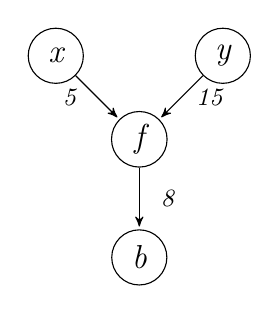
\begin{tikzpicture}
[->,>=stealth',shorten >=1pt,
node distance=1.5cm,
minimum size=7mm,
main node/.style={circle, draw, font=\itshape\large}]

  \node[main node] (1) {x};
  \node[main node] (3) [below right of = 1] {f};
  \node[main node] (2) [above right of = 3] {y};
  \node[main node] (4) [below of = 3] {b};

  \path[every node/.style={font=\itshape\small}]
    
    (1) edge node [left] {5} (3)
    (2) edge node [right] {15} (3)
    (3) edge node [right] {8} (4);
    
\end{tikzpicture}

\end{center}

\caption{A call graph}
\label{callgraph1}

\end{figure}



\end{description}

\begin{flushleft}
Instead, classifying profilers according to the method of data acquisition:
\end{flushleft}


\begin{description}
\item[Event-based profilers] \hfill \\
Some high-level languages and frameworks have they ad-hoc profilers based on
events. For example, \textbf{Java} has \textbf{JVMPI} \textit{(Java Virtual
Machine Profiling Interface)}, while in \textbf{.NET} it's possible to attach a
profiling agent as COM server to a .NET program using the \emph{Profiling APIs}.
These profilers are called \emph{event-based} because statements (of the
relative intermediate language) like function calls (or returns), object
creations (and many others \ldots) have \emph{traps} handled at low-level by the
relative virtual machine which generates \emph{events} and propagates these ones
to the high-level user event-handlers objects.

\item[Statistical profilers] \hfill \\
This kind of profilers work by \emph{sampling} at regular intervals the
\emph{instruction pointer} of target program through \emph{software interrupts}.
This approach, of course, doesn't produce numerically exact data, but allows the
program to run at near full speed. Common profilers of that kind are \textbf{AMD
CodeAnalyst}, \textbf{Apple Shark}, \textbf{Intel VTune} and \textbf{Intel
Parallel Amplifier}.

\item[Instrumentation profilers] \hfill \\
This kind of profilers are used for \emph{native programs}\footnote{A native
program is a program written in a compiled language like \textbf{C},
\textbf{C++}, \textbf{Pascal}: the result of the building is an executable
containing architecture-specific instructions. Instead, non-native programs (aka
managed programs) don't contain binary instructions: they contain
intermediate-language (IL) instructions which only the relative virtual machine
(VM) understand. In order to the program to run, their VM runtime compile IL
instructions into machine specific instructions. \textbf{Java} and \textbf{.NET}
technologies use intermediate languages called relatively \textbf{Bytecode} and
\textbf{MSIL}.} and need to add binary instructions to the target program in
order to ``catch events'' like function calls. Instrumentation profilers can be
classified by the way they ``add instructions'' to the target program:

\begin{description}
\item[Manual]
This approach consists in modifying target program source code adding additional
statements in certain locations. For example, it's possible to add profiling
statements at the beginning of a set of procedures and before every their
\verb|return| statement: this method of collecting data allows building function
call-graphs, call context trees and much more; also, this method can be very
reliable but it requires a considerable amount of work.

\item[Automatic source level] This approach is very similar to the last one but
differs from it in the fact that profiling statements are added automatically by
a tool according to an instrumentation policy.

\item[Compiler assisted] Using a \emph{complier assisted} instrumentation means
that the source code remains intact and is the compiler the one who adds
profiling instructions at compile time. A practical example is \verb|gcc| when
used with \verb|-pg| option: it produces an executable with profiling
instructions but (in the specific case of gcc) they are executed only when the
target program is executed in \emph{profiling mode} by the specific tool
\verb|gprof|.

\item[Binary translation]
This approach consist of adding instructions to an already compiled binary executable.

\item[Runtime instrumentation]
In this case, the additional instructions are added at runtime after program is
loaded in memory or really a little before they are going to be executed by the
cpu. In order to this to happen, another program which has \emph{full control}
of the target one is needed. This approach is used by tools like
\textbf{Valgrind} and \textbf{Intel Pin}\footnote{Pin's official page:
\url{http://www.pintool.org}} which is the tool used for the \textbf{IHPP}
project, so it will be explained in detail later.

\item[Runtime injection] This technique is based on the same idea of the last
one but it an a more \emph{lightweight} approach: substantially it consists of
modifying the target program \emph{text} adding unconditional branch
instructions to helper functions. The tool which does this work doesn't have the
\emph{full control} of the target program but only partial. An example of tool
which belongs to this category is \textbf{DynInst}.

\end{description} 

\item[Profiling through a hypervisor/simulator] \hfill \\
This type of profilers analyze the target program by executing it with no
changes in a kind of \emph{virtual machine} which can have also some ad-hoc
hardware support or it can work by literally emulating every single program
instruction. This approach isn't very common today. Two historical softwares
which adopted this approach were IBM SIMMON and IBM OLIVER.

\end{description}

\chapter{Algorithms and data structures in IHPP}
Since IHPP uses new and not yet published\footnote{The conference in which will be presented the work \emph{k-Calling Context
Profiling}~\cite{kccf} will be held in October 2012, as written here:
\mbox{\url{http://splashcon.org/2012/}}} data structures like $k$-SF and $k$-CCF, at least a basilar explanation of these ones is \emph{strictly} necessary in this paper.
Let's start with an example\footnote{This example, like some other ones in this chapter, was taken, for simplicity, from the article \emph{k-Calling Context Profiling}~\cite{kccf}.}: 

\begin{wrapfigure}[21]{l}{6cm}
\begin{center}
\begin{tabular}{r|l}
\textbf{operation} & \textbf{current context} \\
\hline
start & $\langle$$\rangle$ \\
call(r) & $\langle$r$\rangle$ \\
call(a) & $\langle$r,a$\rangle$ \\
call(b) & $\langle$r,a,b$\rangle$ \\
return & $\langle$r,a$\rangle$ \\
return & $\langle$r$\rangle$ \\
call(c) & $\langle$r,c$\rangle$ \\
call(a) & $\langle$r,c,a$\rangle$ \\
call(b) & $\langle$r,c,a,b$\rangle$ \\
return & $\langle$r,c,a$\rangle$ \\
call(b) & $\langle$r,c,a,b$\rangle$ \\
return & $\langle$r,c,a$\rangle$ \\
return & $\langle$r,c$\rangle$ \\
return & $\langle$r$\rangle$ \\
return & $\langle$$\rangle$ \\
%\hline

\end{tabular}
\caption{an execution trace}
\label{callex1}
\end{center}
\end{wrapfigure}

\mbox{}\\ \mbox{}\\
The figure on the left is an execution trace of a very simple imaginary program; on its right part a very important information is shown: the current \emph{calling context}. 
%
Here it is possible to continue the talk about context-sensitive profiling started in chapter 1: instead of counting the number of activations of a function (which is called \emph{vertex profiling}), in context-sensitive profiling we count the number of activations of a \emph{path}. In order to clearly explain this concept, some formal definitions are 
necessary.

\textbf{Definition 1}: \emph{$k$-calling context}~\cite{kccf}. 
Let $\pi = \langle r,...,v\rangle$ be a calling context of $v$. The k-calling context of $v$
in $\pi$ is the maximal suffix of $\pi$ of length at most $k+1$.

For example, the $2$-context of $(r,c,a,b)$ is $\langle c,a,b\rangle$ and its $0$-context is $\langle b\rangle$ and \emph{not} $\langle\rangle$.

\textbf{Definition 2}: \emph{Path activation}~\cite{kccf}. 
A path $\pi$ of length $q$ in the call graph of the program is activated by 
a \texttt{\textbf{call(}}$v$\texttt{\textbf{)}}
operation if $\pi$ is the $q$-context of $v$ resulting from the \texttt{\textbf{call}} operation.

\textbf{Definition 3}: \emph{$k$-calling context profiling}~\cite{kccf}. Given a trace
of \texttt{\textbf{call}} and \texttt{\textbf{return}} operations, the $k$-(calling) context
profiling problem consists of computing, for each activated path $\pi$ of length $q\le k$, the number $c(\pi)$ of times $\pi$ is activated.

Now, let's see, as a clarifying example, all $k$-contexts for $k=0,1,2,3$ of the execution trace shown in figure~\ref{callex1}:

\begin{figure}[h]
\begin{center}
\begin{tabular}{c|c|c}
\textbf{k value} & \textbf{k-context} & \textbf{activation counter}\\
\hline
0 & $\langle$r$\rangle$* & 1\\
0 & $\langle$a$\rangle$ & 2\\
0 & $\langle$b$\rangle$ & 3\\
0 & $\langle$c$\rangle$ & 2\\
\hline
1 & $\langle$r,a$\rangle$* & 1\\
1 & $\langle$a,b$\rangle$ & 3\\
1 & $\langle$a,c$\rangle$ & 1\\
1 & $\langle$r,c$\rangle$* & 1\\
1 & $\langle$c,a$\rangle$ & 1\\
\hline
2 & $\langle$r,a,b$\rangle$* & 1\\
2 & $\langle$r,a,c$\rangle$* & 1\\
2 & $\langle$r,c,a$\rangle$* & 1\\
2 & $\langle$c,a,b$\rangle$ & 2\\
\hline
3 & $\langle$r,c,a,b$\rangle$* & 2\\

\end{tabular}
\end{center}
\caption{$k$-contexts for various values of $k$.
Note: contexts marketed with (*) are \emph{full} calling contexts.}
\end{figure}

As we can see, for various values of the $k$ parameter there are more or less $k$-contexts with different activation counter values: for $k=0$ they are, simply, the number of times each function is called. This example is too simple to show that but, in general, as $k$ grows, more context information is added but counter values decrease and, for relatively big values of $k$, information made become too specific for any sort analysis so, it is a profiler's user task to choose the \emph{right} $k$-value.

Now, the problem is how to get (in terms of algorithms and data structures) all $k$-contexts 
of a program run for a given value of $k$: a well-known solution is to build a CCT
(\emph{Calling Context Tree}) ``observing'' the execution flow of the program.

\section{The Calling Context Tree}

The CCT of the execution trace considered until now is shown in figure~\ref{cct1}.
It is self-evident that the CCT contains all $k$-contexts for all values of $k$ even if 
it can be not obvious how a CCT is build or how $k$-calling contexts can be extracted from it.

A simple algorithm for building a CCT is:


\begin{figure}[t]

\begin{center}
\scalebox{0.9}{
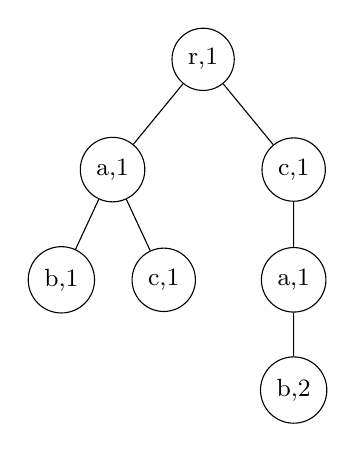
\begin{tikzpicture}[level distance=1.4cm,
  level 1/.style={sibling distance=2.3cm},
  level 2/.style={sibling distance=1.3cm},
  main node/.style={circle,draw,font=\small}]

\node[main node] {r,1}
	child { node[main node] {a,1}
		child { node[main node] {b,1} }
		child { node[main node] {c,1} }
	}
	child { node[main node] {c,1} 
		child { node[main node] {a,1}
			child { node[main node] {b,2} }
		}
	};


\end{tikzpicture}
}
\end{center}

\caption{The CCT of figure~\ref{callex1}. Nodes are labeled in this way: function name, counter.}
\label{cct1}

\end{figure}
\begin{lstlisting}[language=java, morekeywords={function,then},frame=leftline,framesep=10pt]

node treeRoot=null,currentNode=null

function func_call_event_handler(funcType func):

	if (currentNode == null) then 	
		currentNode = new node(func,1) 
		treeRoot=currentNode
		return

	node temp = currentNode.findNodeByFuncInChildren(func)

	if (temp == null) then
		temp = new node(func,1)
		currentNode.addChildren(temp)
	else
		temp.incrementCounter()

	currentNode=temp

function func_ret_event_handler():

	if (currentNode.getParent() != null) then
		currentNode=currentNode.getParent()

\end{lstlisting}

The above code should be self-explaining due to its Java-like style.
The algorithm for extracting $k$-contexts from a CCT is a little more articulated 
and its pseudo-code will not be shown here but the idea is: given a CCT and a node $n$ of it, it is possible to get the $k$-context of $n$ taking the first (or at most) $k$ nodes from the path which joins $n$ with the root node; doing this for every node and summing counters of all identical paths is enough for collecting all $k$-contexts of a CCT.

\section{The k-Calling Context Forest}

As proved in \emph{k-Calling Context Profiling}~\cite{kccf}, building (and handling) a CCT for a relatively long running program is impractical and often useless.
A much better data structure for handling $k$-contexts is \emph{$k$-CCF}: 
the idea on which it is based is to have a \emph{forest} formed by 
a tree (of at most $k$ levels) \emph{for each} function. 

\begin{figure}[h]

\begin{center}
\scalebox{0.8}{
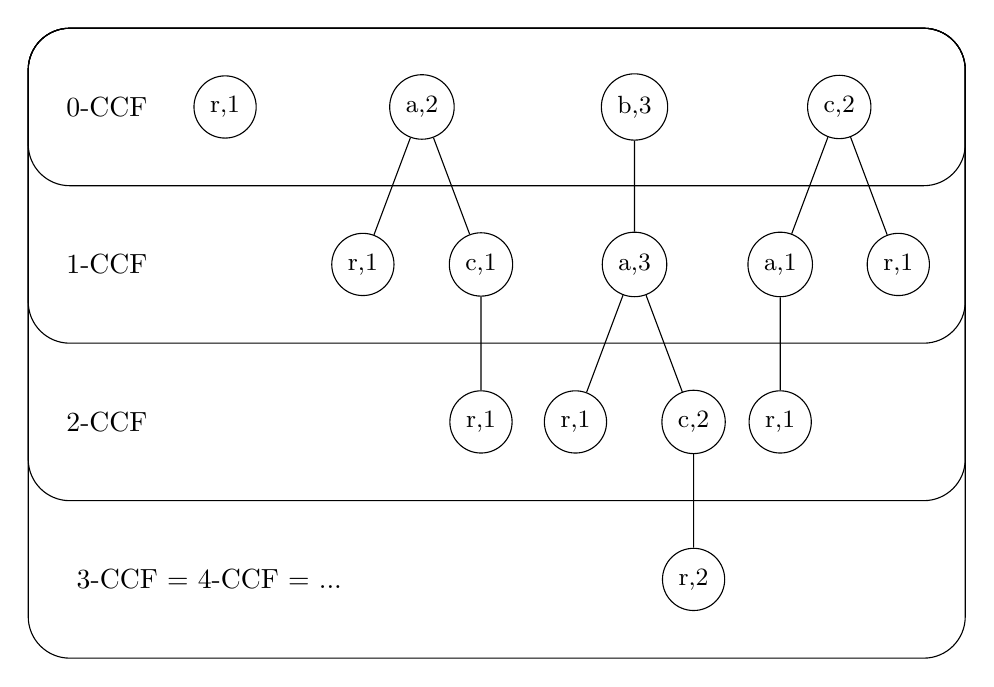
\begin{tikzpicture}[level distance=2.0cm,
  level 1/.style={sibling distance=1.5cm},
  level 2/.style={sibling distance=1.5cm},
  main node/.style={circle,draw,font=\small}]
  

  \node[main node] at (0, 0) {r,1};

  \node[main node] at (2.5, 0) {a,2} 
    child {
	   node[main node] {r,1}
    }
	child {
		node[main node] {c,1}
		child { node[main node]{r,1} }
	};


  \node[main node] at (5.2, 0) {b,3}
  child {
		node[main node] {a,3}
		child { 
			node[main node] {r,1}
		}
		child {
			node[main node] {c,2}
			child { node[main node] {r,2} }
		}
  };

  \node[main node] at (7.8, 0) {c,2}
  child {
		node[main node] {a,1}
		child { node[main node]{r,1} }
  }
  child { node[main node] {r,1} };

  \draw [rounded corners=15pt] (-2.5,-1) rectangle (9.4,1);
  \draw [rounded corners=15pt] (-2.5,-3) rectangle (9.4,1);
  \draw [rounded corners=15pt] (-2.5,-5) rectangle (9.4,1);
  \draw [rounded corners=15pt] (-2.5,-7) rectangle (9.4,1);

  \node at (-1.5,0) {$0$-CCF};
  \node at (-1.5,-2) {$1$-CCF};
  \node at (-1.5,-4) {$2$-CCF};
  \node at (-0.2,-6) {$3$-CCF = $4$-CCF = ...};

\end{tikzpicture}
}
\end{center}

\caption{$k$-CCF relative to CCT in fig.~\ref{cct1} for various values of $k$.}
\label{kccf1}

\end{figure}

The interpretation of fig.~\ref{kccf1} is simple: for $k=0$ there is no context
information and only one node per function is present; its counter shows the number of times that function has been called during the program execution. For $k=1$, every function has as children its callers, for example, $a()$ has been called $2$ times: 1 by $r()$ and 1 by $c()$. This reasoning can be extended for greater values of $k$ with the remark that 
there is always a maximum $k$-value which produces a full context-sensitive information 
(in this example, that value of $k$ is $3$): greater values of $k$ have no effect on the output. 

\subsection{The join operation}

\textbf{Definition 4} \emph{Tree join}~\cite{kccf}. 
The join of two labeled trees $T_1$ and $T_2$, denoted as 
\texttt{\textbf{join(}}$T_1$\texttt{\textbf{,}}$T_2$\texttt{\textbf{)}}, 
is the minimal labeled forest $F$ such that $F$ contains a root-label path $\pi$ if and 
only if $T_1$ or $T_2$ contain $\pi$.

\begin{figure}[h]

\begin{center}
\scalebox{0.9}{

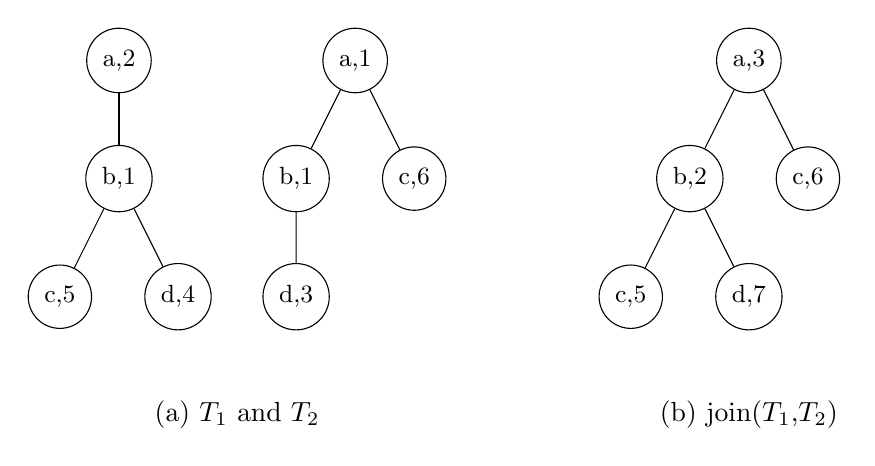
\begin{tikzpicture}[level distance=1.5cm,
  level 1/.style={sibling distance=1.5cm},
  level 2/.style={sibling distance=1.5cm},
  main node/.style={circle,draw,font=\small}]
  
  \node[main node] at (0,0) {a,2}
  child { 
		node[main node] {b,1}
		child {node[main node] {c,5}}
		child {node[main node] {d,4}}
  };

  \node[main node] at (3, 0) {a,1}
  child {
		node[main node] {b,1}
		child {node[main node] {d,3}}
  }
  child {
		node[main node] {c,6}
  };

  \node[main node] at (8, 0) {a,3}
  child {
		node[main node] {b,2}
		child {node[main node] {c,5}}
		child {node[main node] {d,7}}
  }
  child {node[main node] {c,6}};

  \node at (1.5, -4.5) { (a) $T_1$ and $T_2$ };
  \node at (8, -4.5) { (b) join($T_1$,$T_2$) };

\end{tikzpicture}
}
\end{center}

\caption{An example of the tree-join operation}
\label{join1}
\end{figure}

\subsection{The formal definition of k-CCF}

asdj askjd lkajd lkadj lkqdj lkad akda hda hakdj hakjhdaskjh akjf
fsdhjf ksdhf skjhf kjah kahd kahd kahjd kahjd kqhjqkhje kashj 
adhadk hadkas dkjha skdhja kdhja kdhja dkjhad kjahd kah kahd.

\section{The k-Slab Forest}

\begin{lstlisting}[language=java, 
			morekeywords={function,then,endif},
			frame=leftline,framesep=10pt]

set R
stack S
forest kSF
node top=null,bottom=null

function init:
	S.push( (null,null) )

function func_call_event_handler(funcType func):

	(top,bottom) = S.top()
	
	if ( ( (S.size()-1) mod k ) == 0 ) then
		bottom=top
		node temp = R.find( func )

		if (temp == null) then:
			node n2 = new node( func, 0 )
			kSF.addTree(n2)
			R.add(n2)
			top=n2
		else
			top = temp
		endif

	else

		node temp = top.findNodeByFuncInChildren( func )

		if (temp == null) then
			temp = new node( func, 0 )
			top.addChildren( temp )
		endif

		top = temp

	
	top.incrementCounter()

	if (bottom != null) then
		
		node temp = bottom.findNodeByFuncInChildren( func )
		
		if (temp == null) then
			temp = new node( func, 0 )
			bottom.addChildren( temp )
		endif

		bottom = temp
		bottom.incrementCounter()

	endif

	S.push( (top, bottom) )

function func_ret_event_handler():
	S.pop()

\end{lstlisting}

\chapter{An Intraprocedural Hot Path Profiler}

\chapter{The implementation}

IHPP is a profiler written in C++ and \emph{technically} it's a \emph{plug-in}
for the tool \textbf{Pin} developed by \textbf{Intel}; in the Pin-specific slang,
plug-ins like IHPP are called \emph{pintools}.

\chapter{Case studies}


\chapter{Conclusions}

\bibliography{bibliography}{}
\bibliographystyle{plain}

\end{document}